% chap5.tex (Chapter 5 of the thesis)

\chapter[COMPRESSIBLE NONLINEAR SHALLOW ATMOSPHERE\\ MODEL]{COMPRESSIBLE NONLINEAR SHALLOW ATMOSPHERE MODEL}
\label{chap:5}

In this chapter we consider the solution of the full nonlinear dynamical problem for compressible flow on a rotating sphere with a free-surface. The linearized results of Chapter~\ref{chap:4} are extended, providing detailed information on how the nonlinear progressive wavespeed and amplitude are related. The techniques used to solve the mathematical problem are similar to those used to solve the nonlinear incompressible dynamics problem in Chapter~\ref{chap:3}, and as such an abridged version is presented here with the main focus being on the results, which are shown to differ in some key ways. 

\section{Problem Specification}
\subsection{Conservation Equations}
The equations of motion to be used are those derived in Chapter~\ref{chap:4} for conservation of mass and momentum in the rotating compressible shallow atmosphere system. In dimensionless variables the three conservation equations are given as:
\index{shallow atmosphere equations!non-dimensional compressible}

{\bfseries mass}
\begin{multline}
\left(u_{\scriptscriptstyle \lambda}-\mathrm{Sr}\,c\cos\phi\right)\frac{\partial \, h}{\partial \, \eta} + u_{\scriptscriptstyle \phi}\cos\phi\frac{\partial \, h}{\partial \, \phi} \\ +\frac{(\gamma-1)}{\gamma}h\left[\frac{\partial \, u_{\scriptscriptstyle \lambda}}{\partial \, \eta}+\cos\phi\frac{\partial \, u_{\scriptscriptstyle \phi}}{\partial \, \phi}-u_{\scriptscriptstyle \phi}\sin\phi\right]=0. \label{eq:masscom4non}
\end{multline}
{\bfseries \boldmath$\lambda$ momentum}
\begin{equation}
\left(u_{\scriptscriptstyle \lambda}-\mathrm{Sr}\,c\cos\phi\right)\frac{\partial \, u_{\scriptscriptstyle \lambda}}{\partial \, \eta} + u_{\scriptscriptstyle \phi}\cos\phi\frac{\partial \, u_{\scriptscriptstyle \lambda}}{\partial \, \phi} - \left(\frac{\cos\phi}{\mathrm{Ro}} + u_{\scriptscriptstyle \lambda}\right)u_{\scriptscriptstyle \phi}\sin\phi + \frac{1}{\mathrm{Fr}^2}\frac{\partial \, h}{\partial \, \eta} = 0, \label{eq:lamcom4nonlin}
\end{equation}
{\bfseries \boldmath$\phi$ momentum}
\begin{equation}
\left(u_{\scriptscriptstyle \lambda}-\mathrm{Sr}\,c\cos\phi\right)\frac{\partial \, u_{\scriptscriptstyle \phi}}{\partial \, \eta} + u_{\scriptscriptstyle \phi}\cos\phi\frac{\partial \, u_{\scriptscriptstyle \phi}}{\partial \, \phi} + \left(\frac{\cos\phi}{\mathrm{Ro}} + u_{\scriptscriptstyle \lambda} \right)u_{\scriptscriptstyle \lambda}\sin\phi + \frac{\cos\phi}{\mathrm{Fr}^2}\frac{\partial \, h}{\partial \, \phi} = 0. \label{eq:phicom4nonlin}
\end{equation}
The particular form of \eqref{eq:masscom4non} is the result of specifying that the density and pressure on the free-surface are zero, as in Section~\ref{subsec:probsimp} of the previous chapter. The specific forms for the thermodynamic variables of density and pressure are given by
\begin{equation}
\rho(\hat{r},\eta,\phi) =\left[\frac{(\gamma-1)}{\gamma}\left( \frac{\mbox{M}}{\mbox{Fr}}\right)^2 \left(\hat{a}+\hat{h}(\eta,\phi)-\hat{r}\right) \right]^{\frac{1}{\gamma-1}} \label{eq:dencompnon4}
\end{equation}
and
\begin{equation}
p(\hat{r},\eta,\phi) =\left[\frac{(\gamma-1)}{\gamma}\left( \frac{\mbox{M}}{\mbox{Fr}}\right)^2 \left(\hat{a}+\hat{h}(\eta,\phi)-\hat{r}\right) \right]^{\frac{\gamma}{\gamma-1}}, \label{eq:pcompnon4}
\end{equation}
where $\hat{a}$ is the dimensionless form of the sphere's radius.

\subsection{Mass Specification}
To enable comparison between solutions of the dynamical system given by \eqref{eq:masscom4non}--\eqref{eq:phicom4nonlin} we again use a mass specification condition, so that the total \index{mass specification}mass of the atmosphere is held constant for all solutions calculated. We define a base system mass denoted $M_b$, which is given by \eqref{eq:mbcomp} of Section~\ref{subsec:massspec}. For a general progressive Rossby wave of arbitrary free-surface height $h(\eta,\phi)$, the total mass of fluid contained between the surface of the sphere and the free-surface is given by
\begin{equation}
M_{nl}=\int\limits_0^{2\pi} \int\limits_{-\pi/2}^{\pi/2} \int\limits_{\hat{a}}^{\hat{a}+h(\eta,\phi)} \rho(\hat{r},\phi)\hat{r}^2 \cos\phi\,d\hat{r} d\phi d\eta\,. \label{eq:commassnl}
\end{equation}
Defining 
\begin{align}
\beta &= \frac{(\gamma-1)}{\gamma} \left(\frac{\mathrm{M}}{\mathrm{Fr}} \right)^2, \\
f_3(\eta,\phi) &= \beta(\hat{a}+h(\eta,\phi)),
\end{align}
we can write the integral given by \eqref{eq:commassnl} in the form
\begin{align}
M_{nl} &= \frac{4\kappa (\gamma-1)\beta^{\frac{3-2\gamma}{\gamma-1}}}{\gamma(2\gamma-1)(3\gamma-2)} \times \notag \\
&\quad \int\limits_{0}^{\pi/\kappa} \int\limits_{0}^{\pi/2} h^{\frac{\gamma}{\gamma-1}} \left[2f_3^2(\gamma-1)^2 + 2\beta f_3 (\gamma-1)\gamma \hat{a} + \beta^2\gamma(2\gamma-1)\hat{a}^2 \right]\cos\phi\,d\phi d\eta . \label{eq:mnlcomp}
\end{align}
The nonlinear equation for mass conservation is then given by
\begin{equation}
1-\frac{M_{nl}}{M_b}=0. \label{eq:masscon}
\end{equation}
The complete specification of a nonlinear atmospheric progressive Rossby wave in this compressible model consists of solving \eqref{eq:masscom4non}--\eqref{eq:phicom4nonlin} and \eqref{eq:masscon} subject to some condition defining the amplitude of the wave.

\section{Numerical Solution Method}
\label{sec:nonlinnumer}
\subsection{Series Solution and Algorithm}
\label{subsec:serandalg}
Solutions of the full nonlinear dynamics given in the previous section are sought using \index{Fourier series}Fourier series with similar \index{symmetry conditions}symmetry conditions imposed on the field variables as in Section~\ref{sec:comlinnumer} of Chapter~\ref{chap:4}. Taking these symmetry and boundary conditions into account, the series for the nonlinear problem, using longitudinal truncation $M$ and latitudinal truncation $N$, are given by:
\begin{align}
\ulam(\eta,\phi) &= \omega\cos\phi+\sum_{m=1}^M \sum_{n=1}^N P_{m,n}\cos(\kappa m \eta) \cos\bigl((2n-1)\phi\bigr), \label{eq:Lamseriestruncom}\\
\uphi(\eta,\phi) &= \sum_{m=1}^M \sum_{n=1}^N Q_{m,n}\sin(\kappa m \eta) \sin(2n\phi), \label{eq:Phiseriestruncom}\\
h(\eta,\phi) &= \sum_{n=0}^N H_{0,n}\cos(2 n \phi) \notag \\
&\quad+\sum_{m=1}^{M-1} \sum_{n=1}^N H_{m,n} \cos(\kappa m \eta) (-1)^n \left[ \cos(2n\phi)+\cos\bigl(2(n-1)\phi\bigr) \right]. \label{eq:Hseriestruncom}
\end{align}
Here, \eqref{eq:Hseriestruncom} again uses \index{basis recombination}basis recombination to satisfy boundary conditions at the poles. The nonlinear series \eqref{eq:Lamseriestruncom} for $u_{\lambda}$ now contains the primary zonal flow velocity component. Instead of specifying the polar free-surface height we replace $h_o$ with the single summation term in \eqref{eq:Hseriestruncom} to allow the polar height to be determined from the output of the model.

The solution is \index{forcing!compressible model}forced by either parameterizing the amplitude, denoted $\mathcal{A}$, in terms of one of the unknown coefficients, or specifying the wavespeed $c$. To this end $H_{1,1}$, in the series for $h(\eta,\phi)$, or the wavespeed $c$ is fixed prior to computation, thus removing one of the unknowns from the problem. The majority of computations were performed by specifying $H_{1,1}$, and the second technique of specifying $c$ was reserved for cases where two or more solutions were possible with the same amplitude.

The general solution process consists of finding the set of coefficients $H_{m,n}$, $P_{m,n}$, $Q_{m,n}$ and wavespeed $c$ that make the series \eqref{eq:Lamseriestruncom}--\eqref{eq:Hseriestruncom} a solution of the dynamical system described by \eqref{eq:masscom4non}--\eqref{eq:phicom4nonlin} and \eqref{eq:masscon}. The technique chosen to accomplish this task for the current work was the pseudospectral technique of \index{collocation}collocation in which we require the residuals, obtained by substituting the series into the governing equations, to be zero at every point on a mesh constructed from a finite number of collocation points in the flow field. This is exactly the same technique that was used to solve the incompressible nonlinear dynamics problem of Chapter~\ref{chap:3} and will not be further expanded upon here.

For the collocation points in $\phi$ we restrict computation to the Northern hemisphere since the solution has specific symmetry relative to the equator. In addition, strictly internal points from the domain are chosen, since the specific choice of the basis functions for each series imposes boundary conditions at both $\phi=0$ and $\phi=\pm \pi/2$. Defining
\begin{equation}
\Delta \phi = \frac{\pi}{2(N+1)} \label{eq:delphicom}
\end{equation}
to be the inter-grid point distance in the $\phi$ direction, the $N$ equally-spaced $\phi$-grid points are given by
\begin{equation}
\phi_i = i \Delta \phi, \quad \text{for } i=1,2,\ldots,N. \label{phigridcom}
\end{equation}

The collocation points in $\eta$ can be obtained in a similar manner; however, since we have stipulated a dependence on the wavenumber $\kappa$ we are only free to choose collocation points from $\eta \in [0,\pi/\kappa)$ to avoid linearly dependent rows in the resulting Jacobian matrix. This also accounts for the fact that the Rossby wave is symmetric about its mid-line $\eta=\pi/\kappa$. Defining 
\begin{equation}
\Delta \eta = \frac{\pi}{M\kappa} \label{eq:deletacom}
\end{equation}
to be the inter-grid point distance in the $\eta$ direction, the $M$ equally spaced $\eta$-grid points are given by
\begin{equation}
\eta_j = (j-1) \Delta \eta, \quad \text{for } j=1,2,\ldots,M. \label{etagridcom}
\end{equation}
The set of points taken from all possible $(\eta_j,\phi_i)$ pairs constitutes the \index{collocation mesh}collocation mesh to be used in the numerical solution.

Evaluating each of the three governing dynamical equations \eqref{eq:masscom4non}--\eqref{eq:phicom4nonlin} at each of the collocation mesh points and computing the mass specification condition \eqref{eq:masscon} yields a vector of \index{residual vector}residuals, denoted $\bol{E}(\bol{a})$, of length $3MN+1$, where $\bol{a}$ is a vector comprised of the wavespeed (if it is not the forcing term) and set of unknown coefficients. A damped Newton--Raphson method, as in Section~\ref{sec:NewRap} of Chapter~\ref{chap:3}, is then used to solve the resulting algebraic system, which has the general form
\begin{equation}
\bol{E}(\bol{a}) = \bol{0}.
\end{equation}
The \index{Jacobian matrix}Jacobian matrix, which is required to compute the updating vector in the Newton--Raphson method, is calculated analytically since the Jacobian elements are, in general, easily determined. Additionally, the total residual error, which is used in assessing the convergence of a solution, is computed using the $L^1$ norm.

The starting guess at the set of unknowns $\bol{a}$ in the \index{Newton--Raphson method}Newton--Raphson method is initially determined from the equivalent small amplitude linearized solution given in Section~\ref{sec:comlinnumer} of the previous chapter. Once a small amplitude nonlinear solution has been determined it is then used as the basis for the next solution to be computed but with a slightly modified value of either $c$ or $H_{1,1}$, depending on the type of forcing. This \index{bootstrapping}bootstrapping procedure forms the basis of mapping the wavespeed versus amplitude relationship incrementally.

Computational efficiency is achieved by \index{basis function!caching}caching each of the basis functions and their derivatives with respect to $\eta$ and $\phi$ at each of the collocation mesh points; this approach reduces the computational overhead incurred by repeated function calls to the trigonometric functions. The integral appearing in \eqref{eq:mnlcomp} is evaluated using numerical quadrature. The particular algorithm used is that of adaptive Lobatto quadrature, with Kronrod extension of the Gauss--Lobatto formula, as detailed in Gander \& Gautschi~\cite{Gander:AQR}. The majority of computations were performed on two separate computers, the first being an AMD \index{computer specifications}Athlon(tm) XP 1800+ processor clocked at 1.54~GHz with 512~MB of physical memory clocked at 266~MHz, the second being an Athlon(tm) XP 2800+ processor clocked at 2.08~GHz with 1~GB of dual channel physical memory clocked at 333~MHz.

\subsection{Amplitude Measurement}
\label{subsec:comampmeas}
In order to \index{Amplitude!measurement method}investigate the relationship between the progressive Rossby wavespeed and amplitude, we require a means of defining the amplitude $\mathcal{A}$ of a particular Rossby wave. For a simple periodic wave, the amplitude can be defined as the maximum deviation from the mean position to an extreme point. The problem of measuring Rossby wave amplitude horizontally on a sphere is somewhat more complicated and arbitrary, however. Due to the multitude of wave shapes that are possible there are an infinite number of mean states about which we can measure wave deviation. We must therefore decide which one is appropriate to use. Because Rossby wave activity is predominantly associated with the mid-latitude regions and also because $\phi=\pm \pi/4$ represents the mid-point between the equator and either pole, we choose the mean reference level as the latitude circle located $45^\text{o}$ from the equator in either hemisphere.

In this context, progressive Rossby waves are perturbations from a base zonal Westerly flow, for which the height contours are simply circles of constant $\phi$. The unperturbed free-surface height contours at $\phi=\pm\pi/4$ are taken here as the base level, against which Rossby wave amplitudes are measured. This is identical with the definition of amplitude given in Section~\ref{subsec:ampmeas} of Chapter~\ref{chap:3}.

We again observe that the amplitude will not be the same in both the equator-ward and pole-ward directions, and the difference between the two will increase as the overall wave amplitude grows. Thus to record $\mathcal{A}$ effectively we measure both the equator-ward and pole-ward deflections, again denoted $\mathcal{A}_{e}$ and $\mathcal{A}_{p}$ respectively. Associated with these separate amplitudes we define a simple averaged amplitude, the mean of the two values, to be
\begin{equation}
\mathcal{A}_{ave}=\frac{\mathcal{A}_{e}+\mathcal{A}_{p}}{2}.
\end{equation}
It is important to emphasize that these definitions of amplitude are somewhat arbitrary, although they are a useful way of quantifying transverse amplitudes on a spherical surface.

\section{Solution and Results}

\subsection{Model parameters}
The parameters and \index{parameter specification}constants for the model are again chosen to approximate those of the Earth, as in Section~\ref{subsec:comlinmodpar} of the previous chapter. Specifically, the parameters $a$, $\Omega$ and $g$, as well as the four reference scales $v_{\mbox{\tiny ref}}$, $c_{\mbox{\tiny ref}}$, $p_{\mbox{\tiny ref}}$ and $\rho_{\mbox{\tiny ref}}$ are given by \eqref{eq:avalcom}--\eqref{eq:rhovalcom} respectively. Additionally, the reference height level is defined by \eqref{eq:hrefvalcom} and the ratio of specific heats is given as $\gamma=1.4$. 

For the dimensionless zonal flow parameter $\omega$ we use two specific values; these are the same values used in the incompressible nonlinear model of Section~\ref{subsec:incomparams}. The first value is consistent with the angular speed $\omega$ used in the test set proposed by Williamson~et~al.~\cite{Williamson:STS}. The second value, chosen to be 80\% of the first value, provides a slower value for the super rotation rate. In dimensionless form they are given by
\begin{align}
\omega_1 & = 1.25, \\
\omega_2 & = 1.0.
\end{align}

\subsection[Results for $\kappa=4$, $\omega=1.25$]{Results for \boldmath$\kappa=4$, $\omega=1.25$}
Figure~\ref{fig:CvsAk4w125com} shows the wavespeed $c$ computed for $\kappa=4$ and $\omega=1.25$, for each of the three measures of amplitude $\mathcal{A}_{\text{e}}$, $\mathcal{A}_{\text{p}}$ and $\mathcal{A}_{\text{ave}}$. The truncation levels are $M=15$ and $N=15$ and the error tolerance on the $L^1$ norm of the residual vector was set at $10^{-12}$. The solution curves are comprised of a total of 147 converged results; however, the majority of computations were performed for larger values of the amplitude so as to ascertain the detailed behaviour towards the right end of the graph.

The general characteristics of the solution are quite similar to those of the equivalent incompressible model with similar parameters (see Section~\ref{subsec:incomnlk4w125}). For small amplitude the value of the wavespeed $c$ is appropriately approximated by the linearized solution, which is indicated in the figure. Additionally, as the amplitude increases so does the wavespeed, which is to be expected. 

The main new feature of these results, as opposed to the incompressible results refered to previously, is the addition of a new branch, labeled branch 2 in Figure~\ref{fig:CvsAk4w125com}. The small hook-shaped branch 2 was found by first calculating the solution curve at a lower truncation level of $M=N=10$ and then bootstrapping these results to solutions with more coefficients at a higher truncation level. Only a narrow region of convergence was found; however, the solutions contained along this small branch were all found to converge within the required error tolerance norm of $10^{-12}$. 

\begin{figure}[htbp]
\psfrag{Ap}{\small $\mathcal{A}_{\text{p}}$}
\psfrag{Ae}{\small $\mathcal{A}_{\text{e}}$}
\psfrag{Aave}{\small $\mathcal{A}_{\text{ave}}$}
\psfrag{Wavespeed}{\scriptsize Wavespeed, $c$}
\psfrag{Amplitude}{\scriptsize Amplitude (degrees)}
\psfrag{Linearised}{\scriptsize Linearized solution}
\psfrag{B1}{\scriptsize Branch 1}
\psfrag{B2}{\scriptsize Branch 2}
	\centering
		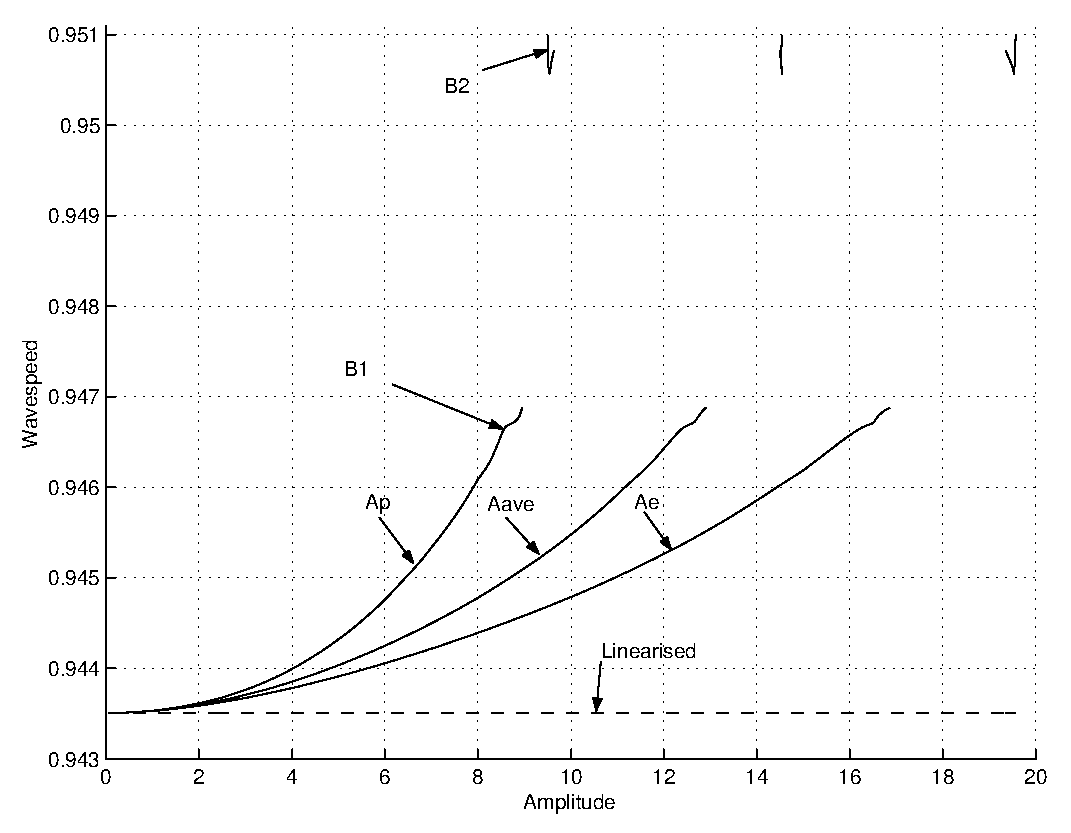
\includegraphics[scale=0.75]{IMAGES/CvsAk4w125com.eps}
	\caption{Compressible wavespeed versus Amplitude for $\kappa=4$ and $\omega=1.25$}
	\label{fig:CvsAk4w125com}
\end{figure}

The separation of the solution curve into two branches again indicates the presence of a \index{resonance!nonlinear}resonant interaction. Attempts were made to find solutions for values of the wavespeed inside the gap between branches 1 and 2 but results indicated that no such solutions exist, or at least are not possible to find using our numerical method. A slight bending-over of the curve at the right end of branch 1 is observed. Identical behaviour was encountered in the incompressible model. Thus it seems likely that the incompressible model might also harbour an additional branch, beyond branch 1, with higher wavespeeds and larger amplitudes, as was conjectured previously in Section~\ref{subsec:incomnlk4w125}.

The free-surface contours at the limiting upper end of branch 2 are show in Figure~\ref{fig:compk4w125fsb2}. To the extent that the difference in the amplitude of solutions lying on the right end of branch 1 and those lying on all of branch 2 is only slight, minimal qualitative difference is seen in the free-surface contours on both branches. Apart from the fact that solutions on branch 2 have greater wavespeeds, which is the main difference between them, a further distinguishing characteristic between the two branches is the formation of a \index{flat-crested wave}flat-crested wave profile in the vicinity of $\phi=\pm \pi/4$ for solutions on the second branch. This shape is visible in Figure~\ref{fig:compk4w125fsb2} as a flat-crested wave for the fifth contour level from the pole. 

\begin{figure}[htbp]
	\centering
		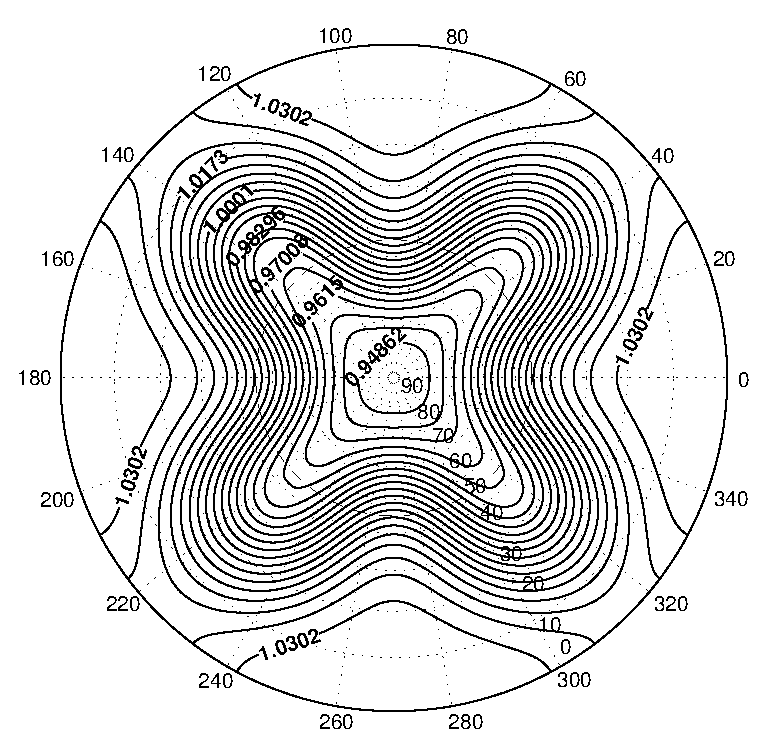
\includegraphics[scale=0.75]{IMAGES/compk4w125fsb2.eps}
	\caption{Compressible free-surface contours at end of branch 2 for $\kappa=4$, $\omega=1.25$.}
	\label{fig:compk4w125fsb2}
\end{figure}

Figure~\ref{fig:comk4w125vecf} shows this flat-crested region in detail, along with the computed velocity vector field. It is seen that this local region of flatness is also reflected in the wind vector. The cause of this feature is unknown but it appears that it would impose a limiting topological constraint for solutions on this branch. It is possible that a third branch exists beyond the second on which solutions would have the property of small localised circulation or ripples in the vicinity of the wave crest. This behaviour would be similar to that first encountered by Wilton~\cite{Wilton:OR}. Attempts were made to find more solution branches using bootstrapping techniques mentioned previously; in all cases no converged solutions were computed with the current numerical method.

\begin{figure}[htbp]
	\centering
		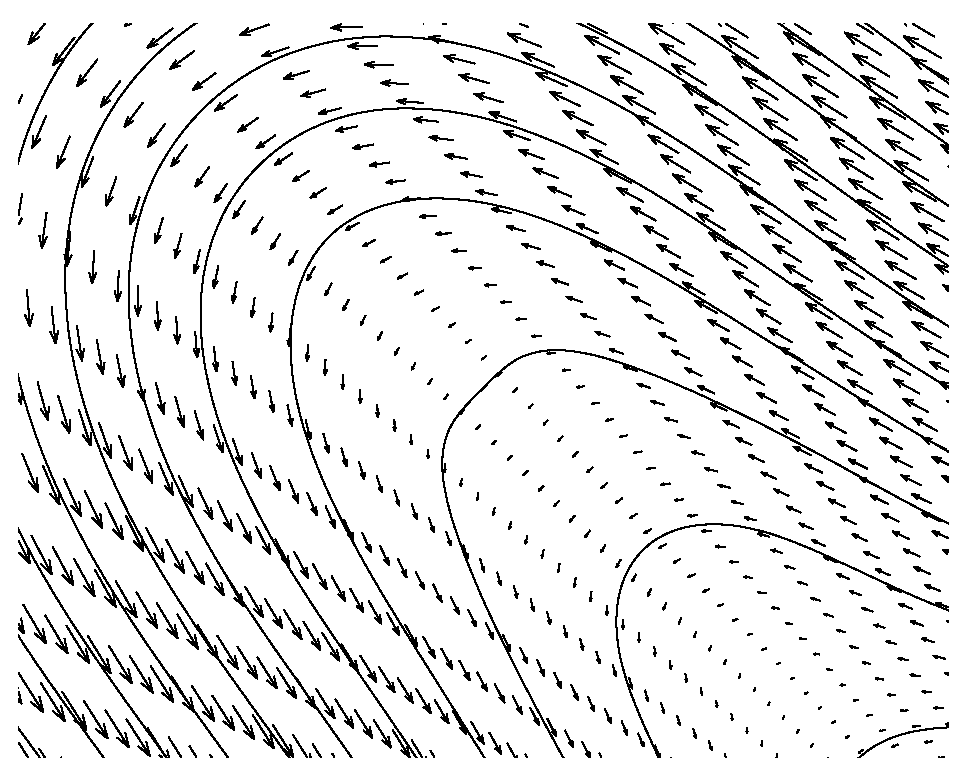
\includegraphics[scale=0.75]{IMAGES/comk4w125vecf.eps}
	\caption{Compressible free-surface contours \index{flat-crested wave}with velocity field at end of branch 2 for $\kappa=4$, $\omega=1.25$.}
	\label{fig:comk4w125vecf}
\end{figure}

\subsection[Results for $\kappa=4$, $\omega=1.0$]{Results for \boldmath$\kappa=4$, $\omega=1.0$}
Figure~\ref{fig:CvsAk4w1com} gives the computed wavespeeds from 197 individual computations using $\kappa=4$ and $\omega=1.0$. Results were obtained by requiring the $L^1$ norm of the residual vector to be less than $10^{-12}$. The truncation levels were again set at $M=N=15$ with little difference observed between solutions obtained with a truncation level of $M=N=10$. Agreement between the nonlinear solution for small amplitude and the linearized result is again observed to be excellent, with the linearization only failing to provide a good estimate of the wavespeed as the amplitude is increased. 

A distinct discontinuous jump is observed in the solution curve, indicating \index{resonance!nonlinear}nonlinear resonance. Of particular note is the peaked, pinched region in the middle of branch 2, which is not present in the equivalent incompressible solution curve (see Figure~\ref{fig:CvsAk4w1}). It is interesting to observe, however, that the incompressible model has a resonance located between branches 2 and 3 and that the qualitative difference between these two branches was minimal. Thus the peaked region in the middle of branch 2 for the compressible model could be seen as a similar phenomenon, except that for the compressible dynamics the behaviour is \index{resonance!damped}damped, so that the effect of the resonance on the solution curve is limited locally.

It is also possible that the segment of the solution curve that has been labelled here as branch 2 is in fact two separate branches. To test whether this claim could be true, the solutions on branch 2 were calculated using a very small amplitude increase each time; in total, over 70 points comprise the computed branch 2 solution. Although the local peaked region was encountered, no break in the continuity of the numerical solution occured, in contrast to the similar case for the incompressible dynamics in which a distinct gap was detected. It therefore seems reasonable to conclude that Branch 2 really is a continuous branch containing a damped resonance, on the basis of the careful numerical solution.

\begin{figure}[tbp]
\psfrag{Ap}{\small $\mathcal{A}_{\text{p}}$}
\psfrag{Ae}{\small $\mathcal{A}_{\text{e}}$}
\psfrag{Aave}{\small $\mathcal{A}_{\text{ave}}$}
\psfrag{Wavespeed}{\scriptsize Wavespeed, $c$}
\psfrag{Amplitude}{\scriptsize Amplitude (degrees)}
\psfrag{Linearised}{\scriptsize Linearized solution}
\psfrag{B1}{\scriptsize Branch 1}
\psfrag{B2}{\scriptsize Branch 2}
	\centering
		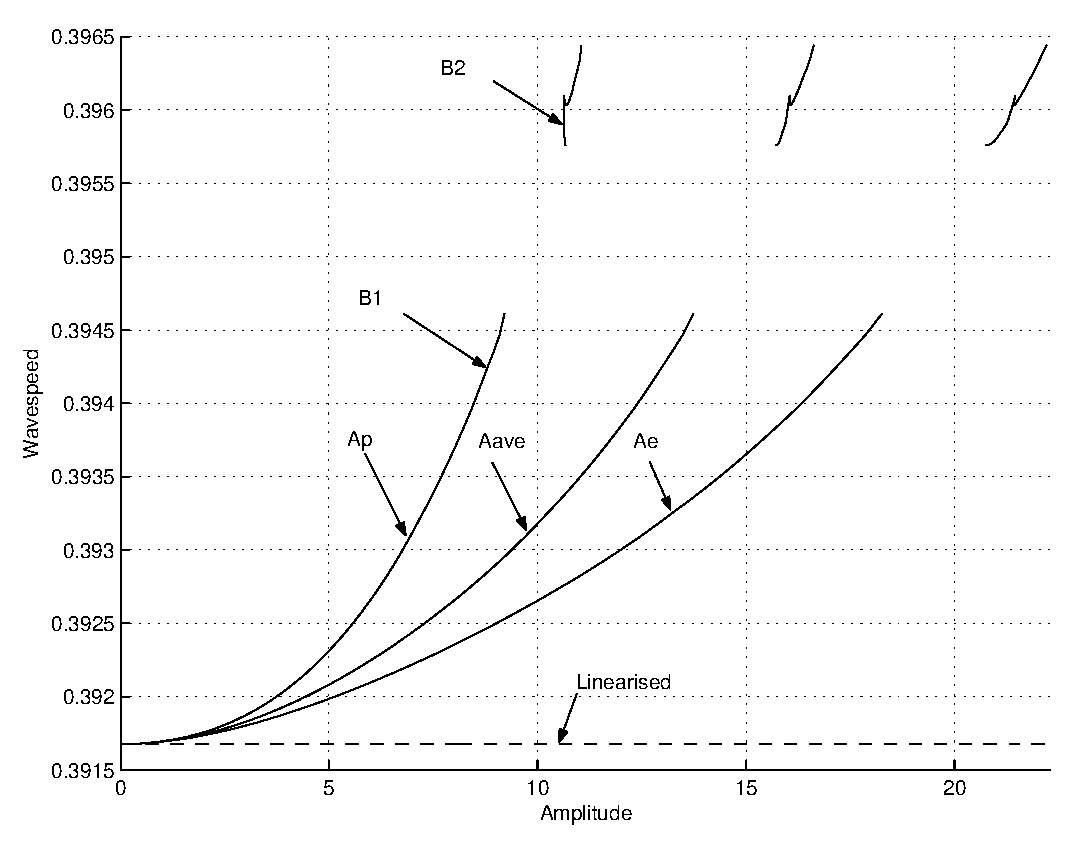
\includegraphics[scale=0.75]{IMAGES/CvsAk4w1com.eps}
	\caption{Compressible wavespeed versus amplitude for $\kappa=4$ and $\omega=1.0$}
	\label{fig:CvsAk4w1com}
\end{figure}

The main distinguishing difference between solutions on branches 1 and 2 can again be exposed by examining the associated velocity vector fields. As in the equivalent incompressible case of Section~\ref{subsec:incomnlk4w1}, it is observed that at no point on branch 1 does the solution contain any \index{stagnation point}stagnation points other than at the poles. For solutions on branch 2, however, there is again the presence of stagnation points on the equator so that the fluid flow is counter to the direction of Rossby wave propagation at certain points in the flow. Because this behaviour is essentially the same as that depicted in Figure~\ref{fig:k4w1fsvvb5end} of Chapter~\ref{chap:3}, no further illustration is given here. It seems reasonable to conjecture that a smooth transition from solutions on branch 1 to solutions on branch 2 is not possible for pure travelling waves and that full nonlinear time dependence is required to study how a wave would make the transition from branch 1 to branch 2, as amplitude is increased. This, in part, explains the existence of the nonlinear resonance between the two distinct branches of the solution curve.

\subsection[Results for $\kappa=5$, $\omega=1.25$]{Results for \boldmath$\kappa=5$, $\omega=1.25$}
We now examine results obtained for $\kappa=5$ and $\omega=1.25$.
\begin{figure}[htbp]
\psfrag{Ap}{\small $\mathcal{A}_{\text{p}}$}
\psfrag{Ae}{\small $\mathcal{A}_{\text{e}}$}
\psfrag{Aave}{\small $\mathcal{A}_{\text{ave}}$}
\psfrag{Wavespeed}{\scriptsize Wavespeed, $c$}
\psfrag{Amplitude}{\scriptsize Amplitude (degrees)}
\psfrag{Linearised}{\scriptsize Linearized solution}
\psfrag{B1}{\scriptsize Branch 1}
\psfrag{B2}{\scriptsize Branch 2}
	\centering
		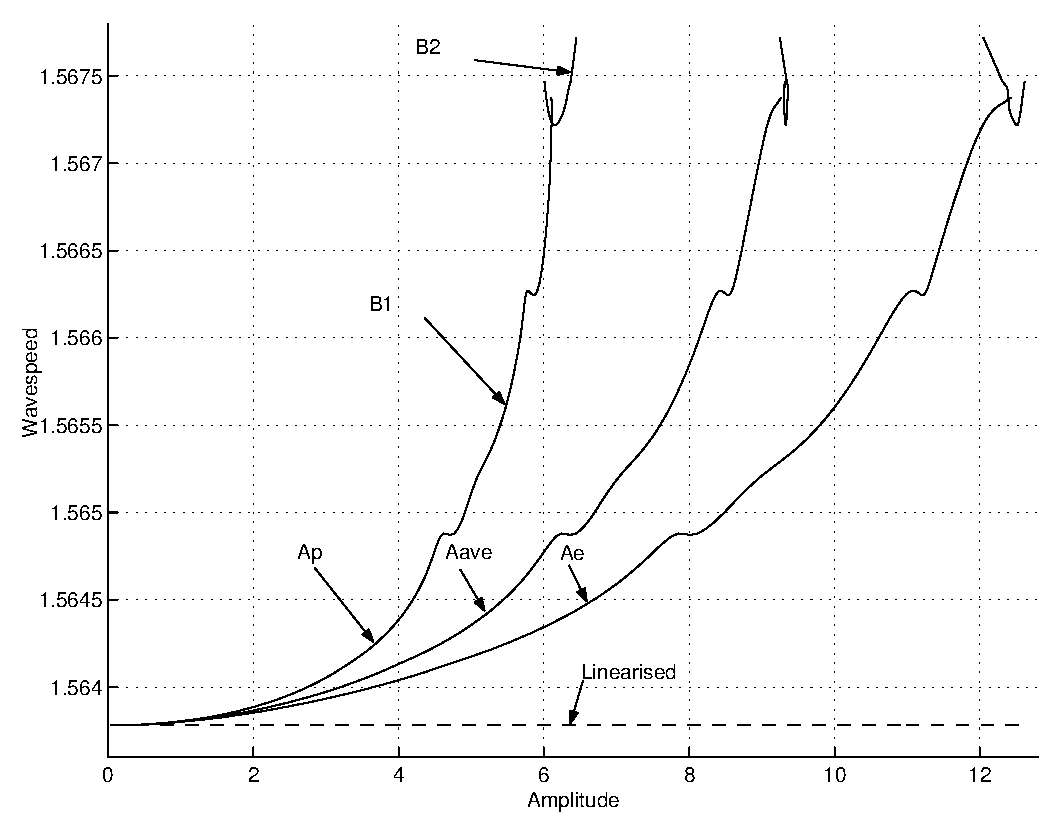
\includegraphics[scale=0.75]{IMAGES/CvsAk5w125com.eps}
	\caption{Compressible wavespeed versus Amplitude for $\kappa=5$ and $\omega=1.25$}
	\label{fig:CvsAk5w125com}
\end{figure}
A total of 262 converged solutions were computed and used to plot the $c$ versus $\mathcal{A}$ relationship in Figure~\ref{fig:CvsAk5w125com}. Note that more points were required here than for previous results because of the detailed structure of the solution curve. Results were obtained with truncation levels of $M=N=15$ and the error tolerance on the $L^1$ norm of the residual vector was set at $10^{-12}$.

The general nature of the graph is seen to be quite similar to that of the incompressible equivalent given in Figure~\ref{fig:CvsAk5w125}, with the linearized solution being a good approximation for small amplitude. However, note the existence of two localised cubic structures on branch 1, as opposed to the single isolated structure for the incompressible case. It was proposed in Section~\ref{subsec:incomnlk5w125} that this behaviour was representative of a type of \index{resonance!damped}damped resonance in which energy exchange between certain wavelengths is taking place in such a maner as to increase the overall amplitude while at the same time reducing the wavespeed. To understand the exact mechanism behind this damping would require, at the very least, careful analytical work beyond the scope of this numerical study. 

Despite this localised reversal of the general trend of the graph, no obvious distinguishing features are visible when the free-surface contours and velocity vector field are examined in the vicinity of these solution regions. Two separate solution branches were again found to exist towards the upper end of the curve when the limiting amplitude-wavespeed combination was approached. However, the qualitative difference between the two branches is minimal and it may be that this second branch is physically unstable, as discussed in Section~\ref{subsec:incomnlk5w125} of Chapter~\ref{chap:2}, or that a greater truncation level is required to resolve the nature of this branch owing to slow convergence of the Fourier series.

\subsection[Results for $\kappa=5$, $\omega=1.0$]{Results for \boldmath$\kappa=5$, $\omega=1.0$}
In this final section we present results for the computed wavespeeds with parameter values given by $\kappa=5$ and $\omega=1.0$, as represented in Figure~\ref{fig:CvsAk5w1com}. The truncation levels were again set at $M=N=15$ and the error tolerance on the $L^1$ norm of the residual vector was set at $10^{-12}$, leading to average individual residual errors of the order of $10^{-15}$ or less. A total of 155 points comprise the makeup of the solution curves. For small amplitudes, the wavespeed is aptly given by the linearized result, as indicated in the figure.

One of the localised cubic structures, seen in the previous set of results, is evident here also, albeit on a much smaller scale, in the vicinity of $c=0.9852$. This behaviour is similar in general to the incompressible results of Section~\ref{subsec:incomnlk5w1}. The main new feature is the introduction of another solution branch as a result of the compressible dynamics. Despite the pinched nature of branch 2, the continuity of the solution along this branch was numerically established by approximately 60 individually converged solutions that failed to exhibit any discontinuous behaviour along the branch. We must therefore conclude, on the basis of numerical evidence, that branch 2 is indeed a continuous solution curve and not two distinct adjacent branches. 

The behaviour of the solution on the second branch again seems to be influenced by some type of damping mechanism. It is not possible to expose the physical nature of this damping mechanism with numerical methods alone. The qualitative difference in the flow fields and free-surface contours for solutions on branch 1 and 2 is quite small, and at no point in the velocity fields of either branch does the fluid flow counter to the direction of progressive Rossby wave motion. Thus no additional stagnation points in the flow field are present. This agrees with the general properties of the equivalent incompressible dynamics of Section~\ref{subsec:incomnlk5w1} of Chapter~\ref{chap:3}.

\begin{figure}[htbp]
\psfrag{Ap}{\small $\mathcal{A}_{\text{p}}$}
\psfrag{Ae}{\small $\mathcal{A}_{\text{e}}$}
\psfrag{Aave}{\small $\mathcal{A}_{\text{ave}}$}
\psfrag{Wavespeed}{\scriptsize Wavespeed, $c$}
\psfrag{Amplitude}{\scriptsize Amplitude (degrees)}
\psfrag{Linearised}{\scriptsize Linearized solution}
\psfrag{B1}{\scriptsize Branch 1}
\psfrag{B2}{\scriptsize Branch 2}
	\centering
		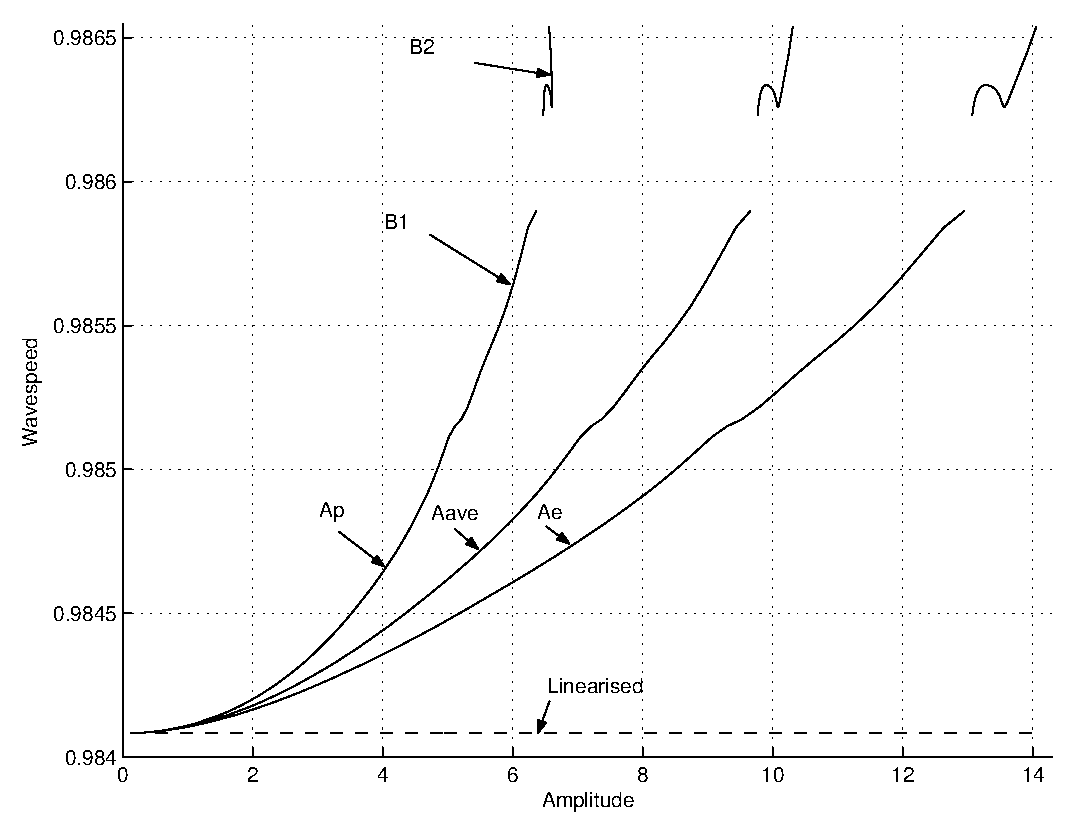
\includegraphics[scale=0.75]{IMAGES/CvsAk5w1com.eps}
	\caption{Compressible wavespeed versus Amplitude for $\kappa=5$ and $\omega=1.0$}
	\label{fig:CvsAk5w1com}
\end{figure}

\section{Closing Remarks}
In this chapter we solved the complete nonlinear equations governing compressible shallow atmosphere free-surface flow. The results obtained were similar to those from the incompressible model with similar parameters; however, small key differences were observed that are attributable to the compressibility of the dynamics. Specifically, it was shown that for all four cases examined, at least two distinct solution branches were found in each instance. The presence of compressibility was observed to damp some instances of resonant behaviour that were encountered in the incompressible model. The cut-off low pressure cells that were computed for $\kappa=4$ and $\omega=1.0$ in the incompressible case were not observed in the compressible model. However, it is suspected that they do still exist and that our numerical scheme was not capable of finding them due to the sensitivity of Newton's method. Attempts to confirm the existence of these cells have thus far been unsuccessful. It is again highly unlikely that numerical methods alone can answer this existence question, and that additional analytical methods may have to be employed. Such an analysis is beyond the scope of the present investigation.
